\documentclass[a4paper,12pt]{article}
%\documentclass[fleqn]{article}

% ---パッケージ---
\usepackage{amsmath,amssymb}    %数式用
\usepackage{tcolorbox}   %囲み枠用(tcolorboxに変更)
\usepackage{geometry}   %余白調節
\usepackage{tikz}  % ← 図を描くためのTikZパッケージ
\geometry{margin=25mm}  %余白を少し狭く
\usetikzlibrary{decorations.pathmorphing,patterns} % バネ・壁の模様

% --- 日本語用パッケージ ---
\usepackage{luatexja}         % 日本語表示に必要
\usepackage{luatexja-fontspec} % フォント指定用

% --- フォント指定(Overleaf標準フォント)---
\setmainjfont{IPAexMincho}  % 明朝体
%\setmainjfont{IPAexGothic}  % ゴシック体にしたい場合

% --- tcolorbox の設定 ---
\tcbset{
    colframe=black,
    colback=white,         % 本文の背景(白)
    boxrule=0.8pt,
    arc=3pt,
    outer arc=3pt,
    boxsep=4pt,
    coltitle=black,
    colbacktitle=gray!20,  % タイトルの背景(グレー)
    fonttitle=\normalsize
}

\begin{document}

% --------------- [21] --------------- 済
\begin{tcolorbox}[title={[21] 単位インパルス応答が\(y(t)=7e^{-2t}+2e^{-3t}\)であるとき,\\ 
    \qquad このシステムの伝達関数を求めよ. }]

    伝達関数は単位インパルス応答\(y(t)\)をラプラス変換して得ることができる.
    \begin{align*}
        \mathcal{L} \left[ y(t) \right] 
        &= 7 \mathcal{L} \left[ e^{-2t} \right]+2 \mathcal{L} \left[ e^{-3t} \right]\\
        &= \frac{7}{s+2} + \frac{2}{s+3}\\
        &= \frac{7s+21+2s+4}{(s+2)(s+3)}\\
        &= \frac{9s+25}{(s+2)(s+3)}\\
        \Leftrightarrow G(s) &= \frac{9s+25}{(s+2)(s+3)}
    \end{align*}

\end{tcolorbox}
% --------------- [22] --------------- 済
\begin{tcolorbox}[title={[22] 単位インパルス応答が\(y(t)=e^{-2t}+3e^{-9t}-4e^{-11t}\)であるとき,\\
    \qquad このシステムの伝達関数を求めよ. }]

    \begin{align*}
        G(s)
        &= \mathcal{L} \left[ y(t) \right] \\
        &= \mathcal{L} \left[ e^{-2t} \right]+3 \mathcal{L} \left[ e^{-9t} \right]-4 \mathcal{L} \left[ e^{-11t} \right]\\
        &= \frac{1}{s+2} + \frac{2}{s+9} - \frac{4}{s+11}\\
        &= \frac{15s+93}{(s+2)(s+9)(s+11)}
    \end{align*}

\end{tcolorbox}
% --------------- [23] --------------- 済
\begin{tcolorbox}[title={[23] 単位ステップ応答が\(y(t)=5e^{-t}-5e^{-7t}\)であるとき,\\
    \qquad このシステムの伝達関数を求めよ. }]

    \qquad 入力信号\(u(t)\)は,大きさ1のステップ関数\(U(s)=\frac{1}{s}\)であるから,
    \begin{align*}
        Y(s)
        &= \mathcal{L} \left[ y(t) \right] \\
        &= 5\mathcal{L} \left[ e^{-t} \right]-5 \mathcal{L} \left[ e^{-7t} \right]\\
        &= \frac{5}{s+1} - \frac{5}{s+7} \\
        &= \frac{30}{(s+1)(s+7)}\\
        \Leftrightarrow G(s) &= \frac{30s}{(s+1)(s+7)} \quad [\because G(s)=\frac{Y(s)}{U(s)}]
    \end{align*}



\vspace{2mm}
\end{tcolorbox}
% --------------- [24] --------------- 済
\begin{tcolorbox}[title={[24] 単位ステップ応答が\(y(t)=12+6t\)であるとき,\\
    \qquad このシステムの伝達関数を求めよ. }]

    \begin{align*}
        Y(s)
        &= \mathcal{L} \left[ y(t) \right] \\
        &= 12\mathcal{L} \left[ 1 \right]+6 \mathcal{L} \left[ t \right]\\
        &= \frac{12}{s} + \frac{6}{s^2} \\
        \Leftrightarrow G(s) &= \frac{12s+6}{s} \quad [\because G(s)=\frac{Y(s)}{U(s)},U(s)=\frac{1}{s}]
    \end{align*}
\end{tcolorbox}
% --------------- [25] --------------- 済
\begin{tcolorbox}[title={[25] 伝達関数が
    \[G(s)=\frac{2}{s^2+3s+2}\]
    \qquad であるときのインパルス応答を求めよ. }]

    \qquad \(Y(s) =G(s)U(s)\) であり,\(U(s)=1\)であるから. 

    \begin{align*}
        Y(s)
        &= \frac{2}{s^2+3s+2}U(s) \\
        &= \frac{2}{(s+1)(s+2)}U(s) \\
        &= \frac{2}{(s+1)(s+2)}\quad [\because U(s)=1]\\
        &= \frac{2}{s+1} - \frac{2}{s+2} \\
        \Leftrightarrow y(t) &= 2e^{-t} - 2e^{-2t}
    \end{align*}

\end{tcolorbox}
% --------------- [26] --------------- 済
\begin{tcolorbox}[title={[26] 伝達関数が
    \[G(s)=\frac{2}{s^2+3s+2}\]
    \qquad であるときのステップ応答を求めよ.}]

    \qquad \(Y(s) =G(s)U(s)\) であり,\(U(s)=\frac{1}{s}\)であるから. 

    \begin{align*}
        Y(s)
        &= \frac{2}{s^2+3s+2}U(s) \\
        &= \frac{2}{s(s+1)(s+2)} \quad [\because U(s)=\frac{1}{s}]\\
        &= \frac{1}{s} - \frac{2}{s+1} + \frac{1}{s+2}\\
        \Leftrightarrow y(t) &=1 - 2e^{-t} + e^{-2t}
    \end{align*}

\end{tcolorbox}
% --------------- [27] --------------- 済
\begin{tcolorbox}[title={[27] 伝達関数が
    \[G(s)=\frac{12s+30}{s^2+8s+15}\]
    \qquad であるときのステップ応答を求めよ. }]

    \qquad \(Y(s) =G(s)U(s)\) であり,\(U(s)=\frac{1}{s}\)であるから. 

    \begin{align*}
        Y(s)
        &= \frac{12s+30}{s^2+8s+15}U(s) \\
        &= \frac{12s+30}{s(s+3)(s+5)} \quad [\because U(s)=\frac{1}{s}]\\
        &= \frac{2}{s} + \frac{1}{s+3} - \frac{3}{s+5}\\
        \Leftrightarrow y(t) &=2 + e^{-3t} - 3e^{-5t}
    \end{align*}

\end{tcolorbox}
% --------------- [28] --------------- 済
\begin{tcolorbox}[title={[28] \(x(t)[m^3/s]\)は,操作バルブ直後の流量を表し,
    長い配管を通って\\
    \qquad \(L[s]\)後に給水場所に到達したとする.\\
    \qquad このとき,\(x(t)\)から給水量\(y(t)\)までの伝達関数を求めよ.}]
    \quad \(y(t)=x(t-L)\) であるから,
    \begin{align*}
    \mathcal{L} \left[ y(t) \right] 
    &= \mathcal{L} \left[ x(t-L) \right] \\
    &= \int_{0}^{\infty} x(t-L)e^{-st}dt \\
    \Leftrightarrow Y(s) &= e^{-Ls}X(s)
    \end{align*}
    \quad ここで\(Y(s)=G(s)X(s)\)であるから,
    \[
    G(s) = \frac{Y(s)}{X(s)} = e^{-Ls}
    \]
\end{tcolorbox}
\newpage
% --------------- [29] --------------- 済
\begin{tcolorbox}[title={[29] 変位\(x_i(t)[m]\)を入力信号,\\
    \qquad ダッシュポットのシリンダの平衡点からの変位\(x_o(t)[m]\)を出力信号\\
    \qquad とみなしたときの伝達関数を求めよ.ただし,\(x_i(0)= 0, x_o(0)=0\)とする.
    \begin{center}
        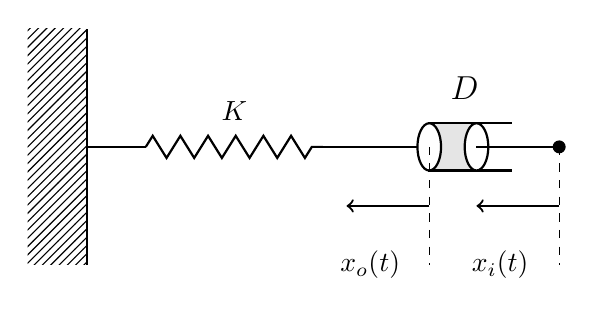
\begin{tikzpicture}[scale=1.5]
          % 固定壁
          \fill[pattern=north east lines] (-0.5,0) rectangle (0,2);
          \draw[thick] (0,0) -- (0,2);
        
          % バネ
          \draw[thick] (0,1) -- (0.5,1);
          \draw[thick, decorate, decoration={zigzag, segment length=10, amplitude=4}] (0.5,1) -- (2,1);
          \node at (1.25,1.3) {$K$};
        
          % --- ダンパー(シリンダー形) ---
    \draw[thick] (2,1) -- (2.9,1); % 棒(変更なし)
    \draw[thick, fill=gray!20] (2.9,0.8) rectangle (3.3,1.2); % 筒の側面
    \draw[thick] (3.3,1.2) -- (3.6,1.2);% 筒の側面(上)
    \draw[thick] (3.3,0.8) -- (3.6,0.8);% 筒の側面(下)
    \draw[thick, fill=white] (2.9,1) ellipse (0.1 and 0.2);   % 左側の端面(楕円)
    \draw[thick, fill=white] (3.3,1) ellipse (0.1 and 0.2);   % 右側の端面(楕円)
    \draw[thick] (3.3,1) -- (4.0,1); % ピストン棒 → 始点を 3.5 → 3.3 に変更
    \node at (3.2,1.5) {\large $D$};
    
    
          % 入力矢印
          \draw[->, thick] (4,0.5) -- (3.3,0.5);
          \node at (3.5,0) {$x_i(t)$};
        
          % 出力矢印
          \draw[->, thick] (2.9,0.5) -- (2.2,0.5);
          \node at (2.4,0) {$x_o(t)$};
        
          % 支点
          \draw[fill] (4,1) circle (0.05);
        
          % 点線
          \draw[dashed] (2.9,1) -- (2.9,0);
          \draw[dashed] (4.0,1) -- (4.0,0);
        \end{tikzpicture}
        \end{center}}]
    
    %解答

    \({x}_o(t),{x}_i(t)\)について運動方程式を立てると,
    \begin{align*}
        \left\{
            \begin{aligned}
                m_o \ddot{x}_o &= -K\,x_o - D\bigl(\dot{x}_o-\dot{x}_i\bigr),\\
                m_i \ddot{x}_i &= D\bigl(\dot{x}_o-\dot{x}_i\bigr) + f(t)
            \end{aligned}
        \right.
    \end{align*}
        ここで入力側にかかる力\(f(t)\)はわからないので,もう一方の式に着目すると,
    \begin{align*}
        &\qquad m_o \ddot{x}_o = -K\,x_o - D\bigl(\dot{x}_o-\dot{x}_i\bigr) \\
        &\therefore \quad m_o \ddot{x}_o + K\,x_o + D \dot{x}_o=D \dot{x}_i \\
        &\therefore \quad \mathcal{L} \left[  m_o \ddot{x}_o + D \dot{x}_o + K\,x_o  \right] 
        =\mathcal{L} \left[ D \dot{x}_i \right] \\
        &\therefore \quad (m_o s^2 + D s + K)\,X_o(s) = D\,s\,X_i(s). \quad [\because x_i(0)= 0, x_o(0)=0 ]\\
        &\therefore \quad G(s) \;=\;\frac{X_o(s)}{X_i(s)}
        \;=\;\frac{D\,s}{m_o s^2 + D s + K}\\
        &\therefore \quad G(s) = \frac{D\,s}{ D s + K} \quad [m_o=0 \text{とした} ]
    \end{align*}

\end{tcolorbox}
\newpage
% --------------- [30] --------------- 済
\begin{tcolorbox}[title={[30] 外力\(f(t)[N]\)を図の方向に考え,平衡点からの変位\(x(t)[m]\)を出力信号\\
    \qquad とみなしたときの伝達関数を求めよ. 
    \begin{center}
        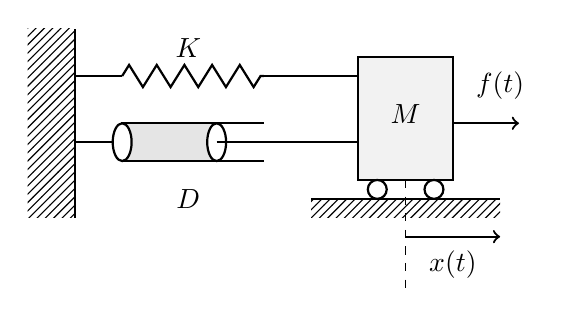
\begin{tikzpicture}[scale=1.2]
          % 固定壁
          \fill[pattern=north east lines] (-0.5,0) rectangle (0,2);
          \draw[thick] (0,0) -- (0,2);
        
          % バネ
          \draw[thick] (0,1.5) -- (0.5,1.5);
          \draw[thick, decorate, decoration={zigzag, segment length=10, amplitude=4}] (0.5,1.5) -- (2,1.5);
          \draw[thick] (2,1.5) -- (3.5,1.5);
          \node at (1.2,1.8) {$K$};
        
          % ダンパー(シリンダー形式)
          \draw[thick] (0,0.8) -- (0.5,0.8); % 棒
          \draw[thick, fill=gray!20] (0.5,0.6) rectangle (1.5,1.0); % 筒の側面
          \draw[thick] (1.5,1.0) -- (2,1.0); % 筒の上
          \draw[thick] (1.5,0.6) -- (2,0.6); % 筒の下
          \draw[thick, fill=white] (0.5,0.8) ellipse (0.1 and 0.2); % 左端面
          \draw[thick, fill=white] (1.5,0.8) ellipse (0.1 and 0.2); % 右端面
          \draw[thick] (1.5,0.8) -- (3,0.8); % ピストン棒
          \node at (1.2,0.2) {$D$};
        
          % 質量M
          \draw[thick, fill=gray!10] (3,0.4) rectangle (4,1.7);
          \node at (3.5,1.1) {$M$};
          % ローラー追加
            \draw[thick] (3.2,0.3) circle (0.1);
            \draw[thick] (3.8,0.3) circle (0.1);
    
        
          % 床
          \draw[thick] (2.5,0.2) -- (4.5,0.2);
          \fill[pattern=north east lines] (2.5,0) rectangle (4.5,0.2);
        
          % 座標
          \draw[->, thick] (3.5,-0.2) -- (4.5,-0.2);
          \node at (4,-0.5) {$x(t)$};
          \draw[dashed] (3.5,0.4) -- (3.5,-0.8);
        
          % 外力
          \draw[->, thick] (4,1) -- (4.7,1);
          \node at (4.5,1.4) {$f(t)$};
        \end{tikzpicture}
        \end{center}
        }]

        %解答

        \(x(t)\)に関する運動方程式より
        \begin{align*}
            &\qquad M\ddot{x} =f(t) -Kx - D \dot{x} \\
            &\therefore \quad M\ddot{x} + Kx + D \dot{x} =f(t) \\
            &\therefore \quad \mathcal{L} \left[ M\ddot{x} + D \dot{x} + Kx\right] 
            =\mathcal{L} \left[ f(t) \right] \\
            &\therefore \quad (M s^2 + D s + K)\,X(s) = F(s) \quad [\because x_i(0)= 0, x_o(0)=0 ]\\
            &\therefore \quad G(s) \;=\;\frac{X(s)}{F(s)}
            \;=\;\frac{1}{M s^2 + D s + K}\\
        \end{align*}

\end{tcolorbox}
% --------------- [31] --------------- 済
\begin{tcolorbox}[title={[31] 平衡点からの変位として,図中の\(x_i(t)[m]\)と\(x_o(t)[m]\)を考える.\\
    \qquad \(x_i(t)\)を入力信号,\(x_o(t)[m]\) を出力信号とみなしたときの伝達関数を求めよ.
    \begin{center}
        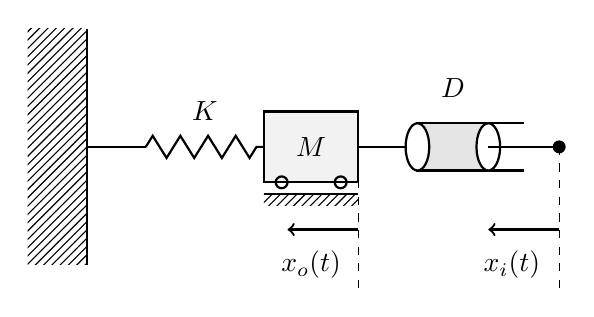
\begin{tikzpicture}[scale=1.5]
          % 固定壁
          \fill[pattern=north east lines] (-0.5,0) rectangle (0,2);
          \draw[thick] (0,0) -- (0,2);
    
          % バネ
          \draw[thick] (0,1) -- (0.5,1);
          \draw[thick, decorate, decoration={zigzag, segment length=10, amplitude=4}] (0.5,1) -- (1.5,1);
          \node at (1,1.3) {$K$};
        
          % 質量M
          \draw[thick, fill=gray!10] (1.5,0.7) rectangle (2.3,1.3);
          \node at (1.9,1) {$M$};
          % ローラー
          \draw[thick] (1.65,0.7) circle (0.05);
          \draw[thick] (2.15,0.7) circle (0.05);
          % 地面
          \draw[thick] (1.5,0.6) -- (2.3,0.6);
          \fill[pattern=north east lines] (1.5,0.5) rectangle (2.3,0.6);
        
          % ダンパー
          \draw[thick] (2.3,1) -- (2.8,1); % 棒
          \draw[thick, fill=gray!20] (2.8,0.8) rectangle (3.4,1.2); % 筒
          \draw[thick] (3.4,1.2) -- (3.7,1.2); % 筒上
          \draw[thick] (3.4,0.8) -- (3.7,0.8); % 筒下
          \draw[thick, fill=white] (2.8,1) ellipse (0.1 and 0.2);
          \draw[thick, fill=white] (3.4,1) ellipse (0.1 and 0.2);
          \draw[thick] (3.4,1) -- (4,1); % ピストン棒
          \node at (3.1,1.5) {$D$};
        
          % 入力矢印
          \draw[->, thick] (4,0.3) -- (3.4,0.3);
          \node at (3.6,0) {$x_i(t)$};
        
          % 出力矢印
          \draw[->, thick] (2.3,0.3) -- (1.7,0.3);
          \node at (1.9,0) {$x_o(t)$};
        
          % 支点
          \draw[fill] (4,1) circle (0.05);
        
          % 点線
          \draw[dashed] (2.3,1) -- (2.3,-0.2);
        \draw[dashed] (4,1) -- (4,-0.2);
        \end{tikzpicture}
        \end{center}
        }]

        \({x}_o(t),{x}_i(t)\)について運動方程式を立てると,
    \begin{align*}
        \left\{
            \begin{aligned}
                M\ddot{x}_o &= -K\,x_o - D\bigl(\dot{x}_o-\dot{x}_i\bigr),\\
                m\ddot{x}_i &= D\bigl(\dot{x}_o-\dot{x}_i\bigr) + f(t)
            \end{aligned}
        \right.
    \end{align*}
        ここで入力側にかかる力\(f(t)\)はわからないので,もう一方の式に着目すると,
    \begin{align*}
        &\qquad M\ddot{x}_o = -K\,x_o - D\bigl(\dot{x}_o-\dot{x}_i\bigr) \\
        &\therefore \quad M\ddot{x}_o + K\,x_o + D \dot{x}_o=D \dot{x}_i \\
        &\therefore \quad \mathcal{L} \left[  M\ddot{x}_o + D \dot{x}_o + K\,x_o  \right] 
        =\mathcal{L} \left[ D \dot{x}_i \right] \\
        &\therefore \quad (M s^2 + D s + K)\,X_o(s) = D\,s\,X_i(s). \quad [\because x_i(0)= 0, x_o(0)=0 ]\\
        &\therefore \quad G(s) \;=\;\frac{X_o(s)}{X_i(s)}
        \;=\;\frac{D\,s}{M s^2 + D s + K}\\
    \end{align*}


\end{tcolorbox}
% --------------- [32] --------------- 済
\begin{tcolorbox}[title={[32] 粘性減衰係数\(D_1[N \cdot s /m]\)のダッシュポットのピストンの平衡点からの変位\\
    \qquad \(x_i(t)[m]\)を入力信号,粘性減衰係数\(D_1[N \cdot s /m]\)のダッシュポットのピストン \\
    \qquad の平衡点からの   変位\(x_o(t)[m]\) を出力信号としたときの伝達関数を求めよ.
\begin{center}
  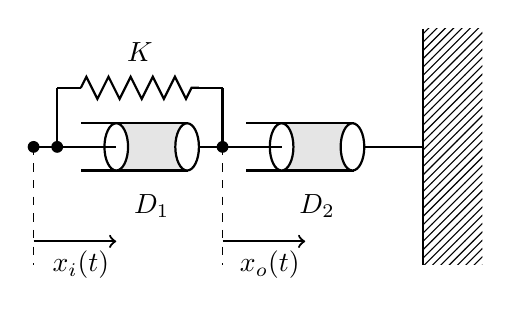
\begin{tikzpicture}[scale=1.5]
    % 固定壁
    \fill[pattern=north east lines] (4,0) rectangle (4.5,2);
    \draw[thick] (4,2) -- (4,0);
  
    % ダンパ D2
    \draw[thick, fill=gray!20] (2.8,0.8) rectangle (3.4,1.2);
    \draw[thick] (2.8,1.2) -- (2.5,1.2);
    \draw[thick] (2.8,0.8) -- (2.5,0.8);
    \draw[thick, fill=white] (2.8,1) ellipse (0.1 and 0.2);
    \draw[thick, fill=white] (3.4,1) ellipse (0.1 and 0.2);
    \draw[thick] (2,1) -- (2.8,1);
    \draw[thick] (3.5,1) -- (4,1);
    \node at (3.1,0.5) {$D_2$};
  
    % ダンパ D1
    \draw[thick, fill=gray!20] (1.4,0.8) rectangle (2.0,1.2);
    \draw[thick] (1.4,1.2) -- (1.1,1.2);
    \draw[thick] (1.4,0.8) -- (1.1,0.8);
    \draw[thick, fill=white] (1.4,1) ellipse (0.1 and 0.2);
    \draw[thick, fill=white] (2.0,1) ellipse (0.1 and 0.2);
    \draw[thick] (0.7,1) -- (1.4,1);
    \node at (1.7,0.5) {$D_1$};
  
    % バネ K
    \draw[thick] (0.9,1) -- (0.9,1.5);
    \draw[thick] (0.9,1.5) -- (1.1,1.5);
    \draw[thick, decorate, decoration={zigzag, segment length=8, amplitude=4}] (1.1,1.5) -- (2.1,1.5);
    \draw[thick] (2.1,1.5) -- (2.3,1.5);
    \draw[thick] (2.3,1) -- (2.3,1.5);
    \node at (1.6,1.8) {$K$};
  
    % 接点
    \fill (0.7,1) circle (0.05);
    \fill (0.9,1) circle (0.05);
    \fill (2.3,1) circle (0.05);

  
    % 点線(基準線)
    \draw[dashed] (0.7,1) -- (0.7,0);
    \draw[dashed] (2.3,1) -- (2.3,0);
  
    % 入力 x₁(t)
    \draw[->, thick] (0.7,0.2) -- (1.4,0.2);
    \node at (1.1,0) {$x_{i}(t)$};
  
    % 出力 x₂(t)
    \draw[->, thick] (2.3,0.2) -- (3,0.2);
    \node at (2.7,0) {$x_{o}(t)$};
    \end{tikzpicture}
    \end{center}}]

    \({x}_o(t),{x}_i(t)\)について運動方程式を立てると,
    \begin{align*}
        \left\{
            \begin{aligned}
                M\ddot{x}_i &= K(x_o - x_i) + D_1\bigl(\dot{x}_o-\dot{x}_i\bigr)+ f(t),\\
                m\ddot{x}_o &= - K(x_o - x_i) - D_1\bigl(\dot{x}_o-\dot{x}_i\bigr) - D_2 \dot{x}_o\\
            \end{aligned}
        \right.
    \end{align*}
        ここで入力側にかかる力\(f(t)\)はわからないので,もう一方の式に着目すると,
    \begin{align*}
        &\qquad m\ddot{x}_o = - K(x_o - x_i) - D_1\bigl(\dot{x}_o-\dot{x}_i\bigr) - D_2 \dot{x}_o \\
        &\therefore \quad m\ddot{x}_o + (D_1 +D_2) \dot{x}_o + K\,x_o = D_1 \dot{x}_i + K x_i\\
        &\therefore \quad \mathcal{L} \left[  m\ddot{x}_o + (D_1 +D_2) \dot{x}_o + K\,x_o  \right] 
        =\mathcal{L} \left[ D_1 \dot{x}_i + K x_i \right] \\
        &\therefore \quad \left\{m s^2 + (D_1+D_2) s + K\right\}\,X_o(s) 
        = (D_1s+K)X_i(s). \quad [\because x_i(0)= 0, x_o(0)=0 ]\\
        &\therefore \quad G(s) \;=\;\frac{X_o(s)}{X_i(s)}
        \;=\;\frac{D_1s+K}{m s^2 + (D_1+D_2) s + K}\\
        &\therefore \quad G(s) \;
        \;=\;\frac{D_1s+K}{(D_1+D_2) s + K}\quad [\because m=0\text{とした}]\\
    \end{align*}

\end{tcolorbox}
\newpage
% --------------- [33] ---------------
\begin{tcolorbox}[title={[33] 平衡点からの変位として,図中の\(x_i(t)[m]\)と\(x_o(t)[m]\)を考える. \\
    \qquad \(x_i(t)[m]\)を入力信号,\(x_o(t)[m]\)を出力信号とみなしたときの伝達巻子を求めよ.\\
    \qquad 台車は摩擦なく床を動くものとする.すべての変数の初期値はゼロである.
    
    \begin{center}
        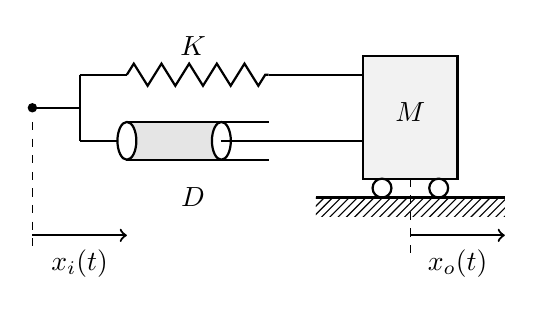
\begin{tikzpicture}[scale=1.2]
          % バネ
          \draw[thick] (0,1.5) -- (0.5,1.5);
          \draw[thick, decorate, decoration={zigzag, segment length=10, amplitude=4}] (0.5,1.5) -- (2,1.5);
          \draw[thick] (2,1.5) -- (3.5,1.5);
          \node at (1.2,1.8) {$K$};
        
          % ダンパー(シリンダー形式)
          \draw[thick] (0,0.8) -- (0.5,0.8); % 棒
          \draw[thick, fill=gray!20] (0.5,0.6) rectangle (1.5,1.0); % 筒の側面
          \draw[thick] (1.5,1.0) -- (2,1.0); % 筒の上
          \draw[thick] (1.5,0.6) -- (2,0.6); % 筒の下
          \draw[thick, fill=white] (0.5,0.8) ellipse (0.1 and 0.2); % 左端面
          \draw[thick, fill=white] (1.5,0.8) ellipse (0.1 and 0.2); % 右端面
          \draw[thick] (1.5,0.8) -- (3,0.8); % ピストン棒
          \node at (1.2,0.2) {$D$};
        
          % 質量M
          \draw[thick, fill=gray!10] (3,0.4) rectangle (4,1.7);
          \node at (3.5,1.1) {$M$};
          % ローラー追加
            \draw[thick] (3.2,0.3) circle (0.1);
            \draw[thick] (3.8,0.3) circle (0.1);
    
          % 床
          \draw[thick] (2.5,0.2) -- (4.5,0.2);
          \fill[pattern=north east lines] (2.5,0) rectangle (4.5,0.2);
        
          % 座標
          \draw[->, thick] (3.5,-0.2) -- (4.5,-0.2);
          \node at (4,-0.5) {$x_o(t)$};
          \draw[dashed] (3.5,0.4) -- (3.5,-0.4);
    
          \draw[->, thick] (-0.5,-0.2) -- (0.5,-0.2);
          \node at (0,-0.5) {$x_i(t)$};
          \draw[dashed] (-0.5,1) -- (-0.5,-0.4);
    
          \draw[thick] (0,0.8) -- (0,1.5);
          \draw[thick] (0,1.15) -- (-0.5,1.15);
    
          \fill (-0.5,1.15) circle (0.05);
    
        \end{tikzpicture}
        \end{center}}]

\end{tcolorbox}
% --------------- [34] ---------------
\begin{tcolorbox}[title={[34]この系の伝達関数を求めよ.ただし,fは粘性抵抗係数であり,\\
    \qquad 初期条件\(t = 0\)において\(F=0\)
    \begin{center}
        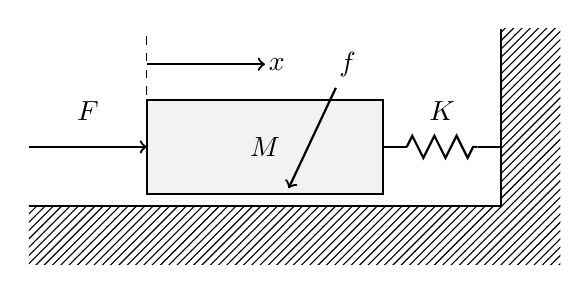
\begin{tikzpicture}[scale=1.5]
          % 固定壁
          \draw[thick] (4,2) -- (4,0.5);
          \fill[pattern=north east lines] (4,0) rectangle (4.5,2);
        
          % バネ
          \draw[thick] (3,1) -- (3.2,1);
          \draw[thick, decorate, decoration={zigzag, segment length=8, amplitude=4}] (3.2,1) -- (3.8,1);
          \draw[thick] (3.8,1) -- (4,1);
          \node at (3.5,1.3) {$K$};
        
          % 質量M
          \draw[thick, fill=gray!10] (1,0.6) rectangle (3,1.4);
          \node at (2,1) {$M$};
    
          %粘性抵抗係数
          \draw[->, thick] (2.6,1.5) -- (2.2,0.65);
          \node at (2.7,1.7) {$f$};
    
          % 地面
          \draw[thick] (0,0.5) -- (4,0.5);
          \fill[pattern=north east lines] (0,0) rectangle (4,0.5);
        
          % 外力
          \draw[->, thick] (0,1) -- (1,1);
          \node at (0.5,1.3) {$F$};
        
          % 点線
          \draw[dashed] (1,0.6) -- (1,2);
        
          % 座標
          \draw[->, thick] (1,1.7) -- (2,1.7);
          \node at (2.1,1.7) {$x$};
        \end{tikzpicture}
        \end{center}}]

\end{tcolorbox}
% --------------- [35] ---------------
\begin{tcolorbox}[title={[35] 長さ\(y_0\)のばねの上端を固定し,下端に質量\(M\)の物体をつり下げたとき,\\
    \qquad ばねの長さが\(y_1\)になって平衡した.\\
    \qquad つぎに,物体に下向きの力\(F(t)\) を加えたとき,物体の平衡状態からの変位を\\
    \qquad \(y\)として運動方程式を作れ.\\
    \qquad ただし物体と側壁との間には,粘性摩擦定数を\(f\)とする.
    \begin{center}
        \begin{tikzpicture}[scale=1.2]
          % 左側(平衡状態)
          \node at (-2,-1)[scale=0.6] {$質量-ばね-まさつ系(平衡状態)$};
    
            %壁
            \draw[thick] (-3,0) -- (-3,4);
            \draw[thick] (-3,4) -- (-1,4);
            \draw[thick] (-1,0) -- (-1,4);
            \fill[pattern=north east lines] (-3.5,0) rectangle (-3,4);
            \fill[pattern=north east lines] (-3.5,4) rectangle (-0.5,4.5);
            \fill[pattern=north east lines] (-1,0) rectangle (-0.5,4);
    
    
            %ばね
            \draw[thick] (-2,1) -- (-2,2);
            \draw[thick, decorate, decoration={coil, segment length=6}] (-2,2) -- (-2,3);
            \draw[thick] (-2,3) -- (-2,4);
            \node at (-2.3,2.5) {$K$};
    
            %重り
            \draw[thick, fill=gray!10] (-2.9,0.2) rectangle (-1.1,1);
            \node at (-2,0.6) {$M$};
    
            %粘性摩擦定数
            \draw[->, thick] (-1.3,0) -- (-1.1,0.6);
            \node at (-1.4,-0.2) {$f$};
    
            %重り
            \draw[dashed] (-2.9,1.2) rectangle (-1.1,2);
    
            %座標
            \draw[dashed] (-4.5,4) -- (-3,4);
            \draw[dashed] (-4.5,1) -- (-2.9,1);
            \draw[dashed] (-4,2) -- (-2.9,2);
    
            \draw[<->,thick] (-3.8,4) -- (-3.8,2);
            \node at (-3.95,3) {$y_0$};
            \draw[<->,thick] (-4.3,4) -- (-4.3,1);
            \node at (-4.45,2.5) {$y_1$};
          
          % 左側(平衡状態)
          \node at (2,-1)[scale=0.6] {$力を加えた場合$};
    
            %壁
            \draw[thick] (3,0) -- (3,4);
            \draw[thick] (3,4) -- (1,4);
            \draw[thick] (1,0) -- (1,4);
            \fill[pattern=north east lines] (3.5,0) rectangle (3,4);
            \fill[pattern=north east lines] (3.5,4) rectangle (0.5,4.5);
            \fill[pattern=north east lines] (1,0) rectangle (0.5,4);
    
    
            %ばね
            \draw[thick] (2,1.3) -- (2,2.2);
            \draw[thick, decorate, decoration={coil, segment length=6}] (2,2.2) -- (2,3.1);
            \draw[thick] (2,3.1) -- (2,4);
            \node at (2.3,2.65) {$K$};
    
            %重り
            \draw[thick, fill=gray!10] (2.9,0.5) rectangle (1.1,1.3);
            \node at (2,0.9) {$M$};
    
            %粘性摩擦定数
            \draw[->, thick] (2.7,0) -- (2.9,0.6);
            \node at (2.6,-0.2) {$f$};
    
            %座標
            \draw[dashed] (0.1,4) -- (1,4);
            \draw[dashed] (0.1,1.3) -- (1.1,1.3);
            \draw[dashed] (2.9,1.3) -- (4,1.3);
    
            \draw[<->,thick] (0.3,4) -- (0.3,1.3);
            \node at (0,2.65) {$y_1$};
    
            \draw[->,thick] (3.8,1.3) -- (3.8,0.5);
            \node at (3.8,0.3) {$y$};
    
            
        
        \end{tikzpicture}
        \end{center}
        }]

\end{tcolorbox}
% --------------- [36] ---------------
\begin{tcolorbox}[title={[36] 質量\(M\)の物体の一端にばねをつけ,\\
    \qquad ばねを力\(F\)で引っ張ったときの運動方程式を作れ.  \\
    \qquad 物体と床面との間の粘性摩擦定数を\(f\)とする.
    
    \begin{center}
        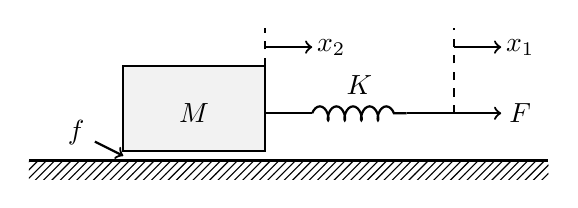
\begin{tikzpicture}[scale=1.2]
          % 地面
          \draw[thick] (-0.5,0) -- (5,0);
          \fill[pattern=north east lines] (-0.5,-0.2) rectangle (5,0);
        
          % 質量M
          \draw[thick, fill=gray!10] (0.5,0.1) rectangle (2,1);
          \node at (1.25,0.5) {$M$};
          \draw[dashed] (2,1.0) -- (2,1.4);
        
          % 摩擦f
          \draw[->,thick] (0.2,0.2) -- (0.5,0.05);
          \node at (0,0.3) {$f$};
        
          % バネ
          \draw[thick] (2,0.5) -- (2.5,0.5);
          \draw[thick, decorate, decoration={coil, segment length=6}] (2.5,0.5) -- (3.5,0.5);
          \node at (3,0.8) {$K$};
          \draw[dashed] (4,0.5) -- (4,1.4);
        
          % 外力
          \draw[->, thick] (3.5,0.5) -- (4.5,0.5);
          \node at (4.7,0.5) {$F$};
        
          % 座標 x2
          \draw[->, thick] (2,1.2) -- (2.5,1.2);
          \node at (2.7,1.2) {$x_2$};
        
          % 座標 x1
          \draw[->, thick] (4,1.2) -- (4.5,1.2);
          \node at (4.7,1.2) {$x_1$};
        \end{tikzpicture}
        \end{center}
        }]

\end{tcolorbox}
% --------------- [37] ---------------
\begin{tcolorbox}[title={[37] 等価変換によってひとつのブロックに簡単化せよ. }]

\end{tcolorbox}
% --------------- [38] ---------------
\begin{tcolorbox}[title={[38] 等価変換によってひとつのブロックに簡単化せよ. }]

\end{tcolorbox}
% --------------- [39] ---------------
\begin{tcolorbox}[title={[39] 等価変換によってひとつのブロックに簡単化せよ. }]

\end{tcolorbox}
% --------------- [40] ---------------
\begin{tcolorbox}[title={[40] 等価変換によってひとつのブロックに簡単化せよ.}]

\end{tcolorbox}
\end{document}